\documentclass[border=4pt]{standalone}
\usepackage{tikz}
\usetikzlibrary{arrows,positioning}
\begin{document}
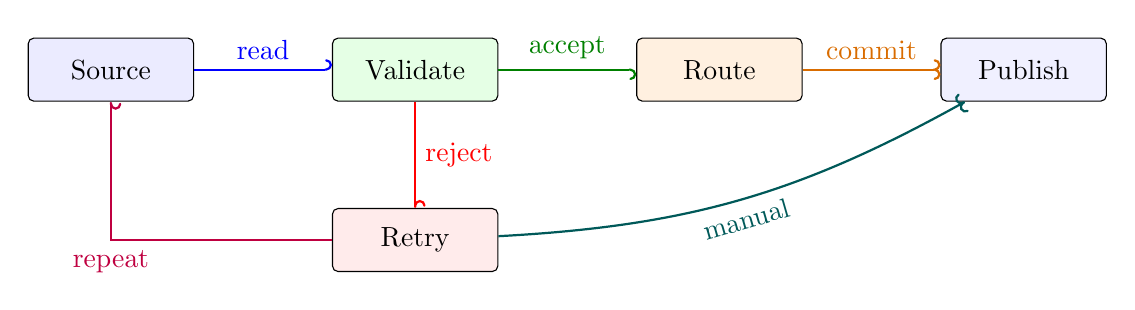
\begin{tikzpicture}[
  node distance=1.35cm and 1.75cm,
  stage/.style={draw,rounded corners=2pt,minimum width=2.1cm,minimum height=8mm,align=center}
]
  \node[stage,fill=blue!8] (source) {Source};
  \node[stage,fill=green!10,right=of source] (validate) {Validate};
  \node[stage,fill=orange!12,right=of validate] (route) {Route};
  \node[stage,fill=blue!6,right=of route] (publish) {Publish};
  \node[stage,fill=red!8,below=of validate] (retry) {Retry};

  \draw[blue,line width=.8pt,-{left hook}] (source) -- node[above]{read} (validate);
  \draw[green!50!black,line width=.8pt,-{right hook}] (validate) -- node[above]{accept} (route);
  \draw[orange!85!black,line width=.8pt,-{hooks}] (route) -- node[above]{commit} (publish);
  \draw[red,line width=.8pt,-{left hook reversed}] (validate) -- node[right]{reject} (retry);
  \draw[purple,line width=.8pt,-{right hook reversed}] (retry) -| node[below]{repeat} (source);
  \draw[teal!70!black,line width=.8pt,-{hooks reversed}] (retry) to[bend right=13] node[below,sloped]{manual} (publish);
\end{tikzpicture}
\end{document}
